\documentclass[12pt]{beamer}

\usetheme[progressbar=frametitle]{metropolis}
\usepackage{appendixnumberbeamer}
\usepackage{algorithm}
\floatname{algorithm}{Algorithm}
\usepackage[noend]{algpseudocode}
\usepackage{booktabs}
\usepackage[scale=2]{ccicons}
\usepackage{multicol}
\newcounter{countitems}
\newcounter{nextitemizecount}
\newcommand{\setupcountitems}{%
  \stepcounter{nextitemizecount}%
  \setcounter{countitems}{0}%
  \preto\item{\stepcounter{countitems}}%
}
\makeatletter
\newcommand{\computecountitems}{%
  \edef\@currentlabel{\number\c@countitems}%
  \label{countitems@\number\numexpr\value{nextitemizecount}-1\relax}%
}
\newcommand{\nextitemizecount}{%
  \getrefnumber{countitems@\number\c@nextitemizecount}%
}
\newcommand{\previtemizecount}{%
  \getrefnumber{countitems@\number\numexpr\value{nextitemizecount}-1\relax}%
}
\makeatother    
\newenvironment{AutoMultiColItemize}{%
\ifnumcomp{\nextitemizecount}{>}{3}{\begin{multicols}{2}}{}%
\setupcountitems\begin{itemize}}%
{\end{itemize}%
\unskip\computecountitems\ifnumcomp{\previtemizecount}{>}{3}{\end{multicols}}{}}
\usepackage{pgfplots}
\usepgfplotslibrary{dateplot}
\usepackage{xspace}
\newcommand{\themename}{\textbf{\textsc{metropolis}}\xspace}

\title{On the automatic planning of healthy and balanced menus}
\date{28 de marzo de 2019}
\author{Alejandro Marrero}
\institute{Máster en Ingeniería Informática}
\titlegraphic{\hfill
\includegraphics[height=1.5cm]{images/original.png}}

\begin{document}

\maketitle

\begin{frame}{Contenidos}
  \setbeamertemplate{section in toc}[sections numbered]
  \tableofcontents[hideallsubsections]
\end{frame}


%%%%%%%%%%%%%%%%%%%%%%%%%%%%%%%%%%%%%%%%%%%%%%%%%%%%%%%%%%%%%%%%%%%%%%%%%%%
% Conceptos previos
\section{Conceptos Previos}

\begin{frame}[fragile]{Optimización Multi-objetivo.}
Formalmente, un problema de optimización multi-objetivo se define como:
\begin{align*}
min\;f(x) & = (f_{1}(x), f_{2}(x), ..., f_{k}(x)), \: x\;\in\chi \\
 g_{i}(x) & \leq 0, \: i = 1, 2, ..., q. \\
 h_{i}(x) & \leq 0, \: i = 1, 2, ..., p.
\end{align*}
donde $x = (x_{1}, x_{2}, ..., x_{n}) \in \mathbb{Z}^{n}$, son las funciones objetivo $f_{i}: \mathbb{Z}^{n} \rightarrow \mathbb{R}, \; i = 1, ..., k$ siendo \textit{n} el número de variables de decisión, $g_{i}: \mathbb{Z}^{n} \rightarrow \mathbb{R}, \; i = ~1, ..., q$ y $h_{i}: \mathbb{Z}^{n} \rightarrow \mathbb{R}, \; i = 1, ..., p$ las funciones de restricción. \\
\begin{itemize}
    \item Método de Optimilidad de Pareto\cite{search, metaheuristics}.
\end{itemize}
\end{frame}

\begin{frame}[fragile]{Computación Evolutiva.}
    \begin{center}
        \texttt{\textbf{\textit{Desarrollan la metáfora de la evolución natural\cite{eiben}.}}}
    \end{center}
    Los Algoritmos Evolutivos Multi-objetivos, \textit{Multi-Objective Evolutionary Algorithms~(MOEAs)} se pueden dividir en:
    \begin{itemize}
        \item MOEAs based on decomposition, i.e., MOEA/D\cite{Zhang2007, Ma2018}.
        \item Pareto-based MOEAs, i.e., NSGA-II\cite{996017} and SPEA-2\cite{Laumanns2001SPEA2}.
        \item Indicator-based MOEAs, i.e., IBEA\cite{IBEA}.
    \end{itemize}
\end{frame}

\begin{frame}[fragile]{Computación Evolutiva.}
 \begin{algorithm}[H]
\begin{algorithmic}[1]
  \State INITIALISE population with random candidate solutions
  \State EVALUATE each candidate
  \While{not StopCriteria satisfied}
    \State SELECT parents
    \State RECOMBINE pairs of parents to obtain the offspring
    \State MUTATE the offspring
    \State EVALUATE new offspring
    \State SELECT individuals from among parents and offspring for the next generation 
  \EndWhile
  \State \textbf{end}
  \end{algorithmic}
    \caption{Esquema General de un Algoritmo Evolutivo.}
\end{algorithm}
\end{frame}

%%%%%%%%%%%%%%%%%%%%%%%%%%%%%%%%%%%%%%%%%%%%%%%%%%%%%%%%%%%%%%%%%%%%%%%%%%%
% Formulación
\section{Formulación del Menu Planning Problem}
\begin{frame}[fragile]{Aproximación Clásica del MPP.}
\begin{center}
        \texttt{\textbf{\textit{Menu Planning Problem~(MPP) es un problema NP-Duro propuesto en 1960\cite{Ngo2016}.}}}
    \end{center}
Hay muchas formulaciones distintas aunque se suelen considerar los objetivos:
    \begin{itemize}
        \item Coste del menú.
        \item Variabilidad.
        \item Tiempo de cocinado.
    \end{itemize}
Multi-objetivo $\rightarrow$ \textit{Problema de la Mochila Multidimensional (MDKP)}.
\end{frame}

\begin{frame}[fragile]{Nueva formulación del MPP.}
    Formulación multi-objetivo del MPP: coste y nivel de repetición.
    \begin{itemize}
        \item Coste del menú.
    \end{itemize}
\[
    min\; C = \sum_{i=1}^{n}{c_{fc_{i}} + c_{sc_{i}} + c_{d_{i}}}
\]
\begin{itemize}
    \item Variabilidad.
\end{itemize}
\[
    min\; L_{Rep} = \sum_{i=1}^{n}{v_{table_{i}} + \frac{p_{fc}}{d_{fc_{i}}} + \frac{p_{sc}}{d_{sc_{i}}} + \frac{p_{ds}}{d_{ds_{i}}} + v_{FG_{i}}}
\]
\end{frame}

\begin{frame}[fragile]{Nueva formulación del MPP.}
Los nutrientes que forman las restricciones: \\
$N = \{$ Ácido Fólico,  Magnesio, Calcio, Potasio, Fósforo, Selenio, Sodio, Hierro, Vitaminas A, B1, B2, B6, B12, C, D y E, Zinc, Yodo, Grasas, Proteínas, Hidratos de Carbono y Energía (Kcal)$\}$ \\

\[
    \forall	 n \in N\; : R_{min_{n}} \leq I_{n} \leq R_{max_{n}}
\]
dónde $I_{n}$ es la cantidad requerida del enésimo-nutriente en el menú.
\end{frame}

\begin{frame}[fragile]{Nueva formulación del MPP.}
Los alimentos están divididos en los siguientes grupos:
\begin{AutoMultiColItemize}
    \item Carne.
    \item Cereales.
    \item Fruta.
    \item Productos Lácteos.
    \item Pescado.
    \item Verdura.
    \item Marisco.
    \item Legumbres.
    \item Pasta.
    \item Otros.
\end{AutoMultiColItemize}
\end{frame}


%%%%%%%%%%%%%%%%%%%%%%%%%%%%%%%%%%%%%%%%%%%%%%%%%%%%%%%%%%%%%%%%%%%%%%%%%%%
% Algoritmos comparados
\section{Algoritmos Comparados}
%%%%%%%%%%%%%%%%%%%%%%%%%%%%%%%%%%%%%%%%%%%%%%%%%%%%%%%%%%%%%%%%%%%%%%%%%%%
% MOEA/D
\begin{frame}[fragile]{Multi-objective Evolutionary Algorithm based on Decomposition~(MOEA/D)}
\begin{center}
        \texttt{\textbf{\textit{Propuesto en 2007 por Qingfu Zhang y Hui Li \cite{Zhang2007}.}}}
    \end{center}
\begin{itemize}
    \item Basado en descomposición. Tchebycheff\cite{Ma2018}.
    \item Establece relaciones entre los sub-problemas mediante vectores de pesos. Vecindarios.
    \item Guiado por un punto de referencia $Z^{*}$.
\end{itemize}
\end{frame}

\begin{frame}[fragile]{MOEA/D}
\begin{algorithm}[H]
\begin{algorithmic}[1]
  \State SetRandomWeightVectors\;
  \State EuclideanDistance\;
  \State GenerateRandomPopulation\;
  \State InitializeZ\;
  \While{not StopCriteria satisfied}
    \ForAll{sub-problem}
      \State l,k = getRandomNeigbours\;
      \State child = reproduce(l, k)\;
      \State child = improve(child)\;
      \State updateZ(child)\;
      \State updateNeighbouringSolutions(child)\;
    \EndFor 
    \EndWhile
    \State \textbf{end}
\end{algorithmic}
\caption{MOEA/D.}
\end{algorithm}
\end{frame}


%%%%%%%%%%%%%%%%%%%%%%%%%%%%%%%%%%%%%%%%%%%%%%%%%%%%%%%%%%%%%%%%%%%%%%%%%%%
% NSGA-II
\begin{frame}[fragile]{Nondominated Sorting Genetic Algorithm II (NSGA-II)}
\begin{center}
        \texttt{\textbf{\textit{Propuesto en 2002 por K. Deb, A. Pratap, S. Agarwal y T. Meyarivan como mejora al NSGA\cite{996017}.}}}
\end{center}
\begin{itemize}
    \item Fast Nondominated Sorting: de $\mathcal{O}(MN^{3})$ a $\mathcal{O}(MN^{2})$.
    \item Operador de selección.
\end{itemize}
\end{frame}
\begin{frame}[fragile]{NSGA-II}
\begin{algorithm}[H]
\begin{algorithmic}[1]
\State P = CreateInitialPopulation(N)\;
\State  FastNondominatedSorting(P)\;
  \While{not StopCriteria satisfied}
    \State BinaryTournamentSelection(P)\;
    \State Q = CreateOffspring(P)\;
    \State R = Combine(P, Q)\;
    \State FastNondominatedSorting(R)\;
    \State P = SelectNIndividuals(R, N)\;
  \EndWhile
  \State \textbf{end}
\end{algorithmic}
\caption{NSGA-II.}
\end{algorithm}
\end{frame}
%%%%%%%%%%%%%%%%%%%%%%%%%%%%%%%%%%%%%%%%%%%%%%%%%%%%%%%%%%%%%%%%%%%%%%%%%%%
% SPEA-2
\begin{frame}[fragile]{Strength Pareto Evolutionary Algorithm 2~(SPEA-2)}
\begin{center}
        \texttt{\textbf{\textit{Publicado en 2001 por Eckart Zitzler, Marco Laumanns y Lothar Thiele\cite{SPEA2}.}}}
\end{center}
\begin{itemize}
    \item Asignación de fitness:
    \begin{enumerate}
        \item Fuerza del individuo \textit{(S)} a partir del número de individuos dominados.
        \item \textit{Raw Fitness} como la suma de S.
        \item Cálculo de la densidad de cada individuo. 
        \item Fitness: $R + D$ para cada individuo.
    \end{enumerate}
    \item Método de truncado de fichero mejorado.
\end{itemize}
\end{frame}

\begin{frame}[fragile]{SPEA-2}
\begin{algorithm}[H]
\begin{algorithmic}[1]
\State P = CreateInitialPopulation(N)\;
\State $\overline{P}$ = CreateEmptyArchive;\;
  \While{not StopCriteria satisfied}
    \State ComputeFitness(P,$\overline{P}$)
    \State EnvironmentalSelection;
    \State BinaryTournamentSelection;
    \State Recombination;
    \State Mutation;
  \EndWhile
  \State \textbf{end}
\end{algorithmic}
\caption{SPEA 2.}
\end{algorithm} 
\end{frame}
%%%%%%%%%%%%%%%%%%%%%%%%%%%%%%%%%%%%%%%%%%%%%%%%%%%%%%%%%%%%%%%%%%%%%%%%%%%%
% Evaluación Experimental
\section{Evaluación Experimental}
\begin{frame}[fragile]{Procedimiento de evaluación}
Usado previamente en \cite{7347400} con un nivel de significación del 5\% y usando el hypervolumen (HV) como métrica:
    \begin{enumerate}
        \item Shapiro-Wilk.
            \begin{enumerate}
                \item Levene.
                \item ANOVA.
                \item Welch.
            \end{enumerate}
        \item Kruskal-Wallis.
    \end{enumerate}
\begin{itemize}
        \item METCO
        \item 25 repeticiones con 1e8 evaluaciones cada una.
        \item 67 platos.
    \end{itemize}
\end{frame}

\begin{frame}[fragile]{Estudio preliminar}
    \begin{center}
        \texttt{\textbf{\textit{Encontrar la mejor configuración del MOEA/D.}}}
    \end{center}
    Entre los parámetros del algoritmo están:
    \begin{itemize}
        \item Tamaño de población: 25, 80, 140, 190, 250.
        \item Tamaño del vecindario: 0.4, 0.3, 0.25, 0.2, 0.16.
        \item Probabilidad de mutación: 0.05.
        \item Probabilidad de cruce: 1.
    \end{itemize}
    Además MPP de \textbf{20 días}.
\end{frame}
\begin{frame}[fragile]{Estudio preliminar}
    \begin{center}
        \texttt{\textbf{\textit{Población: 140 Vecindario: 42}}}
    \end{center}
    \begin{table}[!h]
    \centering
    \resizebox{1\textwidth}{2cm}{%
        \begin{tabular}{|c|c|c|c|c|c|c|c|}
        \hline
        \textbf{Configuration} & \textbf{Min.} & \textbf{Median} & \textbf{Mean} & \textbf{Max.} & \textbf{W} & \textbf{L} & \textbf{Ranking} \\ \hline
       \textbf{ MOEA\_D\_PopSize\_140\_Neihb\_42} & \textbf{0.7161} & \textbf{0.7839} & \textbf{0.7834} & \textbf{0.8435} & 9 & 0 & \textbf{9} \\ \hline
        MOEA\_D\_PopSize\_250\_Neihb\_50 & 0.7270 & 0.7737 & 0.7775 & 0.8213 & 2 & 0 & 2 \\ \hline
        MOEA\_D\_PopSize\_80\_Neihb\_16 & 0.7306 & 0.7787 & 0.7774 & 0.8342 & 2 & 0 & 2 \\ \hline
        MOEA\_D\_PopSize\_140\_Neihb\_35 & 0.7388 & 0.7671 & 0.7728 & 0.8188 & 1 & 0 & 1 \\
        \hline
        \end{tabular}
        }
    \end{table}
\end{frame}
\begin{frame}[fragile]{Variación del Tamaño del Problema.}
    \begin{center}
        \texttt{\textbf{\textit{¿Cómo afecta el tamaño del problema al rendimiento del MOEA/D?}}}
    \end{center}
    \begin{itemize}
        \item Instancias de 5, 10 y 40 días del MPP.
        \item Comparación con los mejores resultados de NSGA-II y SPEA-2.
    \end{itemize}
\end{frame}

\begin{frame}[fragile]{Variación del Tamaño del Problema.}
    \begin{center}
        \texttt{\textbf{\textit{Instancia de 5 días.}}}
    \end{center}
        \begin{table}[!h]
    \centering
    \resizebox{1\textwidth}{2cm}{%
    \begin{tabular}{lcccc}
    \hline
    \textbf{Menu plannings for 5 days} &  &  &  &  \\ \hline
    Configuration & Min. & Std & Mean & Max. \\ \hline
    \textbf{NSGA2\_PopSize\_250\_pm\_0.2\_pc\_0.8} & \textbf{0.956507} & \textbf{0.006186} & \textbf{0.969247} & \textbf{0.977835} \\
    SPEA2\_ps\_100\_ArchSize\_100\_pm\_0.2\_pc\_0.8 & 0.937224 & 0.007334 & 0.951471 & 0.964441 \\
    MOEA\_D\_PopSize\_140\_Neihb\_42 & 0.747678 & 0.030129 & 0.827381 & 0.873078 \\ \hline
    \end{tabular}%
    }
    \end{table}
\end{frame}

\begin{frame}[fragile]{Variación del Tamaño del Problema.}
    \begin{center}
        \texttt{\textbf{\textit{Instancia de 10 días.}}}
    \end{center}
        \begin{table}[!h]
    \centering
    \resizebox{1\textwidth}{2cm}{%
    \begin{tabular}{lcccc}
    \hline
    \textbf{Menu plannings for 10 days} &  &  &  &  \\ \hline
Configuration & Min & Std & Mean & Max. \\ \hline
\textbf{NSGA2\_PopSize\_250\_pm\_0.2\_pc\_0.8} & \textbf{0.934024} & \textbf{0.008141} & \textbf{0.948577} & \textbf{0.961192} \\
SPEA2\_PopSize\_100\_ArchSize\_100\_pm\_0.2\_pc\_0.8 & 0.9237 & 0.008851 & 0.941078 & 0.955088 \\
MOEA\_D\_PopSize\_140\_Neihb\_42 & 0.743725 & 0.030455 & 0.783656 & 0.83404 \\ \hline
    \end{tabular}%
    }
    \end{table}
\end{frame}

\begin{frame}[fragile]{Variación del Tamaño del Problema.}
    \begin{center}
        \texttt{\textbf{\textit{Instancia de 20 días.}}}
    \end{center}
        \begin{table}[!h]
    \centering
    \resizebox{1\textwidth}{2cm}{%
    \begin{tabular}{lcccc}
    \hline
    \textbf{Menu plannings for 20 days} & \multicolumn{1}{l}{} & \multicolumn{1}{l}{} & \multicolumn{1}{l}{} & \multicolumn{1}{l}{} \\ \hline
Configuration & Min. & Std & Mean & Max. \\ \hline
\textbf{SPEA2\_PopSize\_100\_ArchSize\_100\_pm\_0.1\_pc\_0.8} & \textbf{0.906556} & \textbf{0.011438} & \textbf{0.925087} & \textbf{0.945195} \\
NSGA2\_ps\_250\_pm\_0.05\_pc\_0.8 & 0.940483 & 0.014064 & 0.921332 & 0.940483 \\
MOEA\_D\_PopSize\_140\_Neihb\_42 & 0.7161 & 0.03205 & 0.7834 & 0.8435 \\ \hline
    \end{tabular}%
    }
    \end{table}
\end{frame}

\begin{frame}[fragile]{Variación del Tamaño del Problema.}
    \begin{center}
        \texttt{\textbf{\textit{Instancia de 40 días.}}}
    \end{center}
        \begin{table}[!h]
    \centering
    \resizebox{1\textwidth}{2cm}{%
    \begin{tabular}{lcccc}
    \hline
    \textbf{Menu plannings for 40 days} &  &  &  &  \\ \hline
Configuration & Min. & Std & Mean & Max. \\ \hline
\textbf{SPEA2\_ps\_100\_ArchSize\_100\_pm\_0.025\_pc\_0.8} & \textbf{0.891074} & \textbf{0.012357} & \textbf{0.910226} & \textbf{0.929} \\
NSGA2\_ps\_250\_pm\_0.05\_pc\_0.8 & 0.886774 & 0.008034 & 0.9019 & 0.918159 \\
MOEA\_D\_PopSize\_140\_Neihb\_42 & 0.65815 & 0.033453 & 0.716339 & 0.783212
    \end{tabular}%
    }
    \end{table}
\end{frame}

\begin{frame}[fragile]{Variación del Tamaño del Problema.}
\begin{figure}
    \centering
    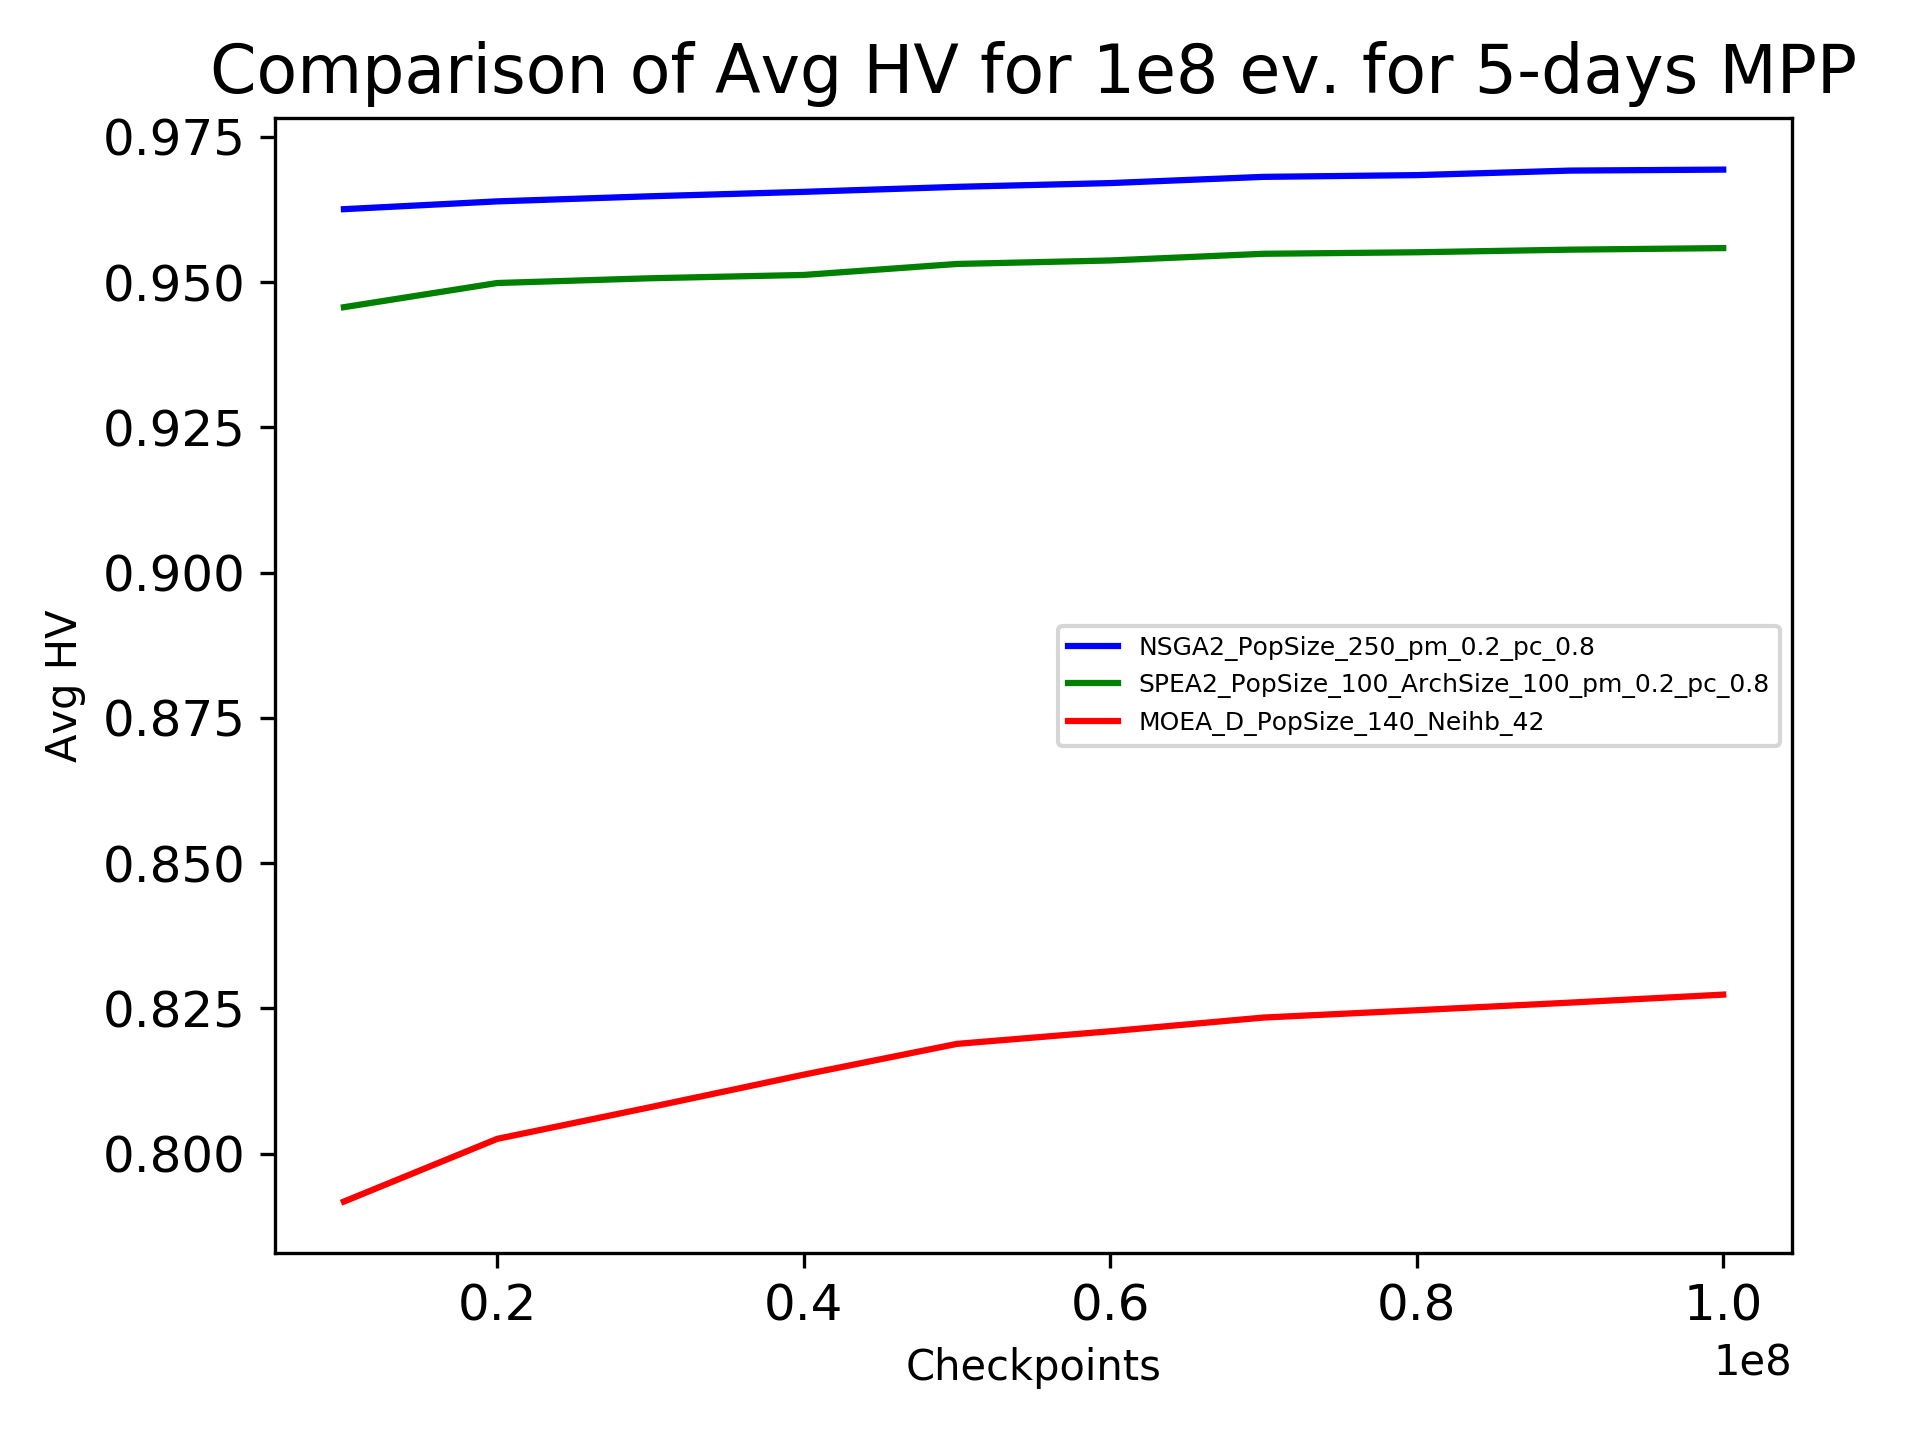
\includegraphics[width=1.0\linewidth]{images/avg_evolution_5_days.png}
\end{figure}
\end{frame}

\begin{frame}[fragile]{Variación del Tamaño del Problema.}
\begin{figure}
    \centering
    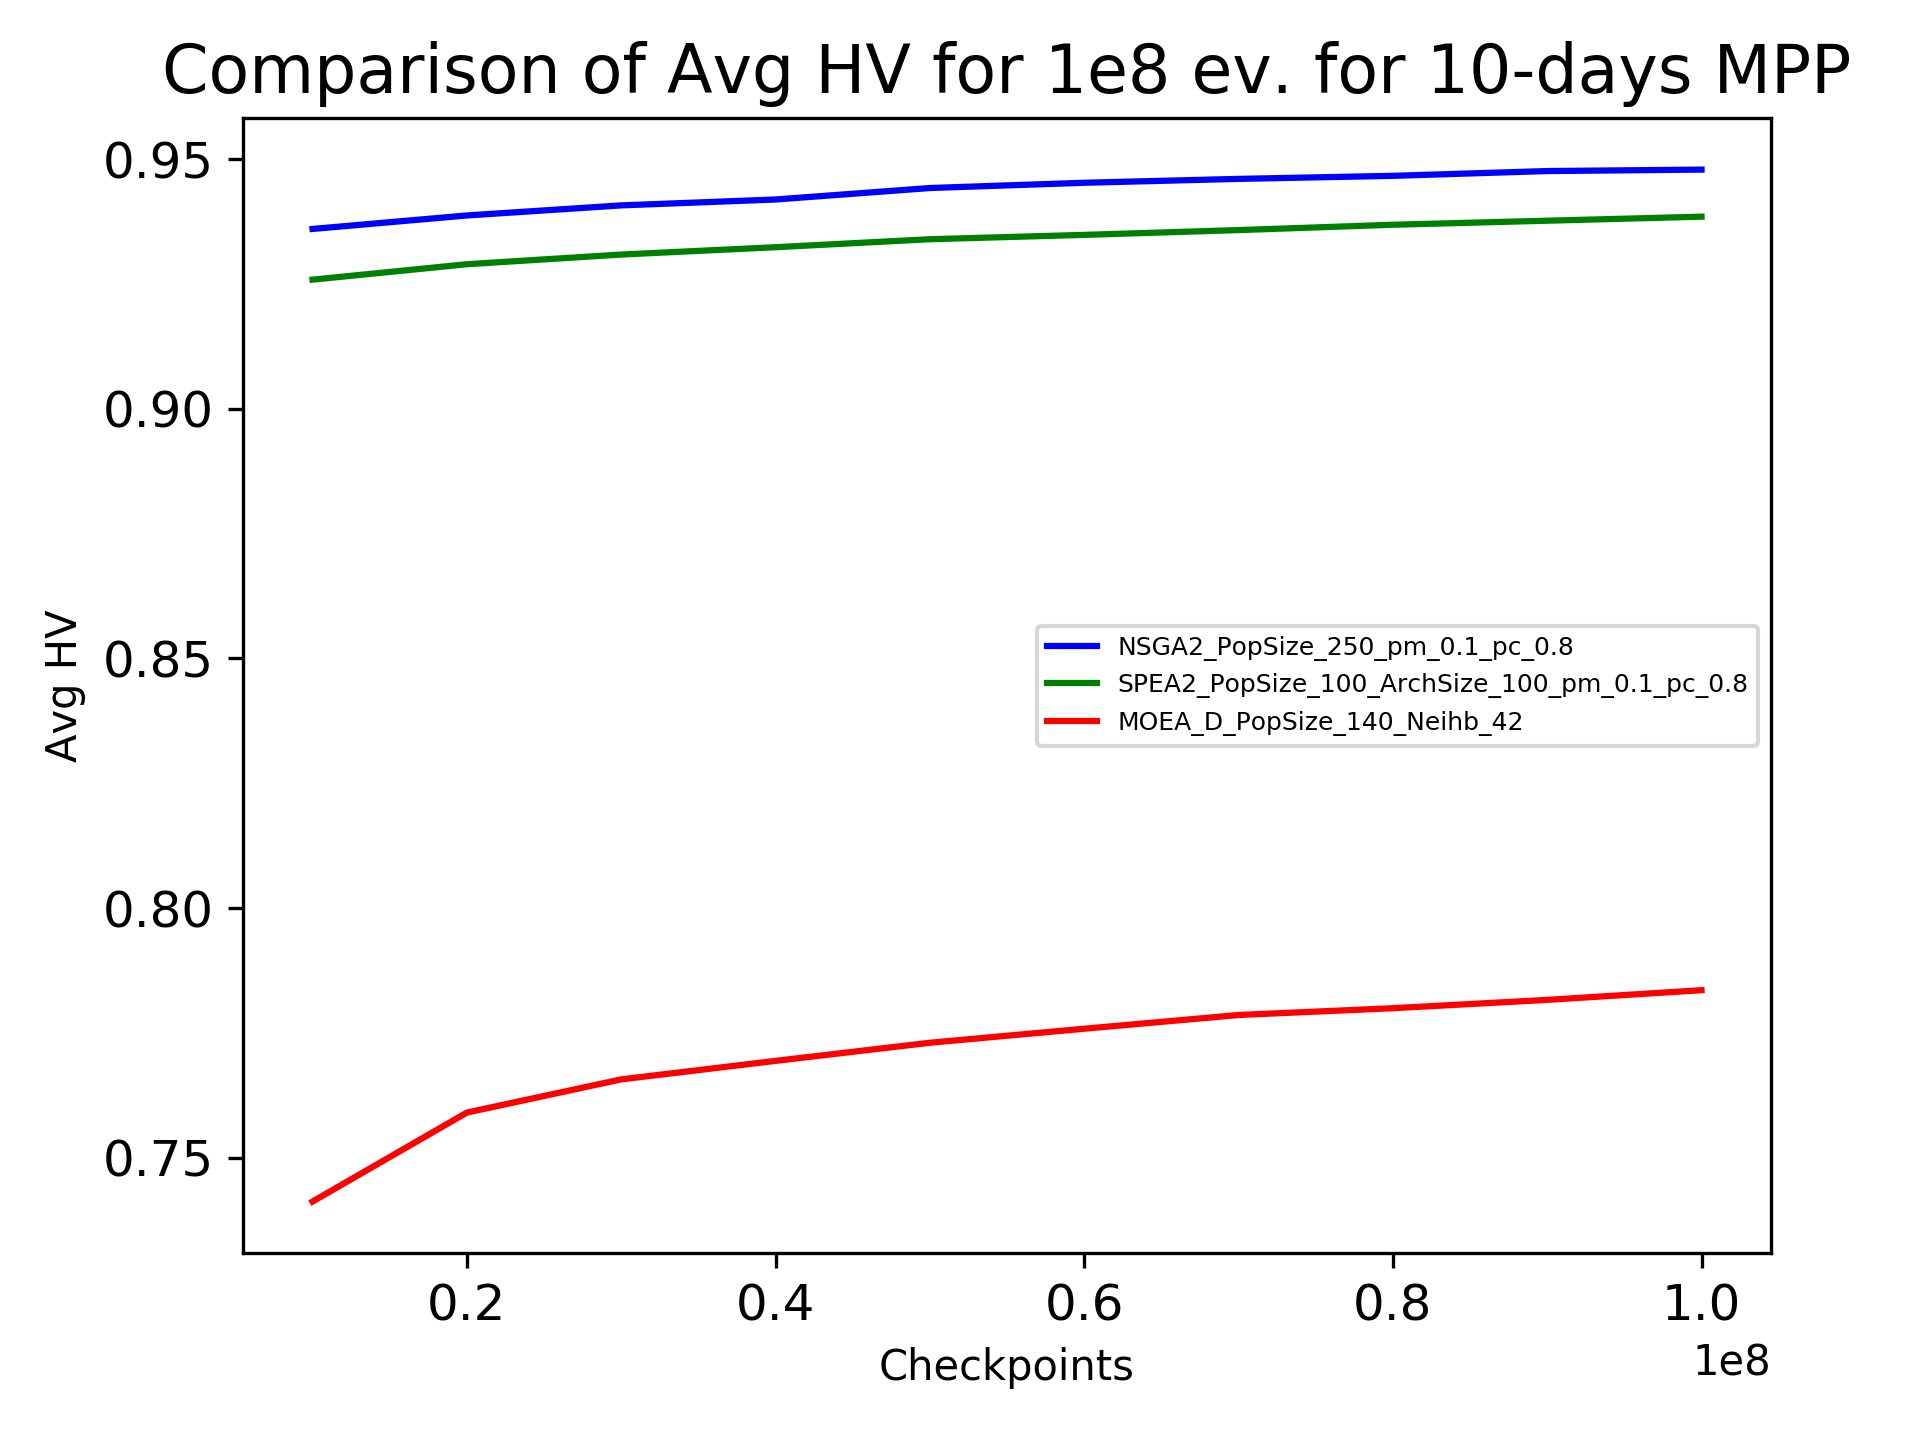
\includegraphics[width=1.0\linewidth]{images/avg_evolution_10_days.png}
\end{figure}
\end{frame}

\begin{frame}[fragile]{Variación del Tamaño del Problema.}
\begin{figure}
    \centering
    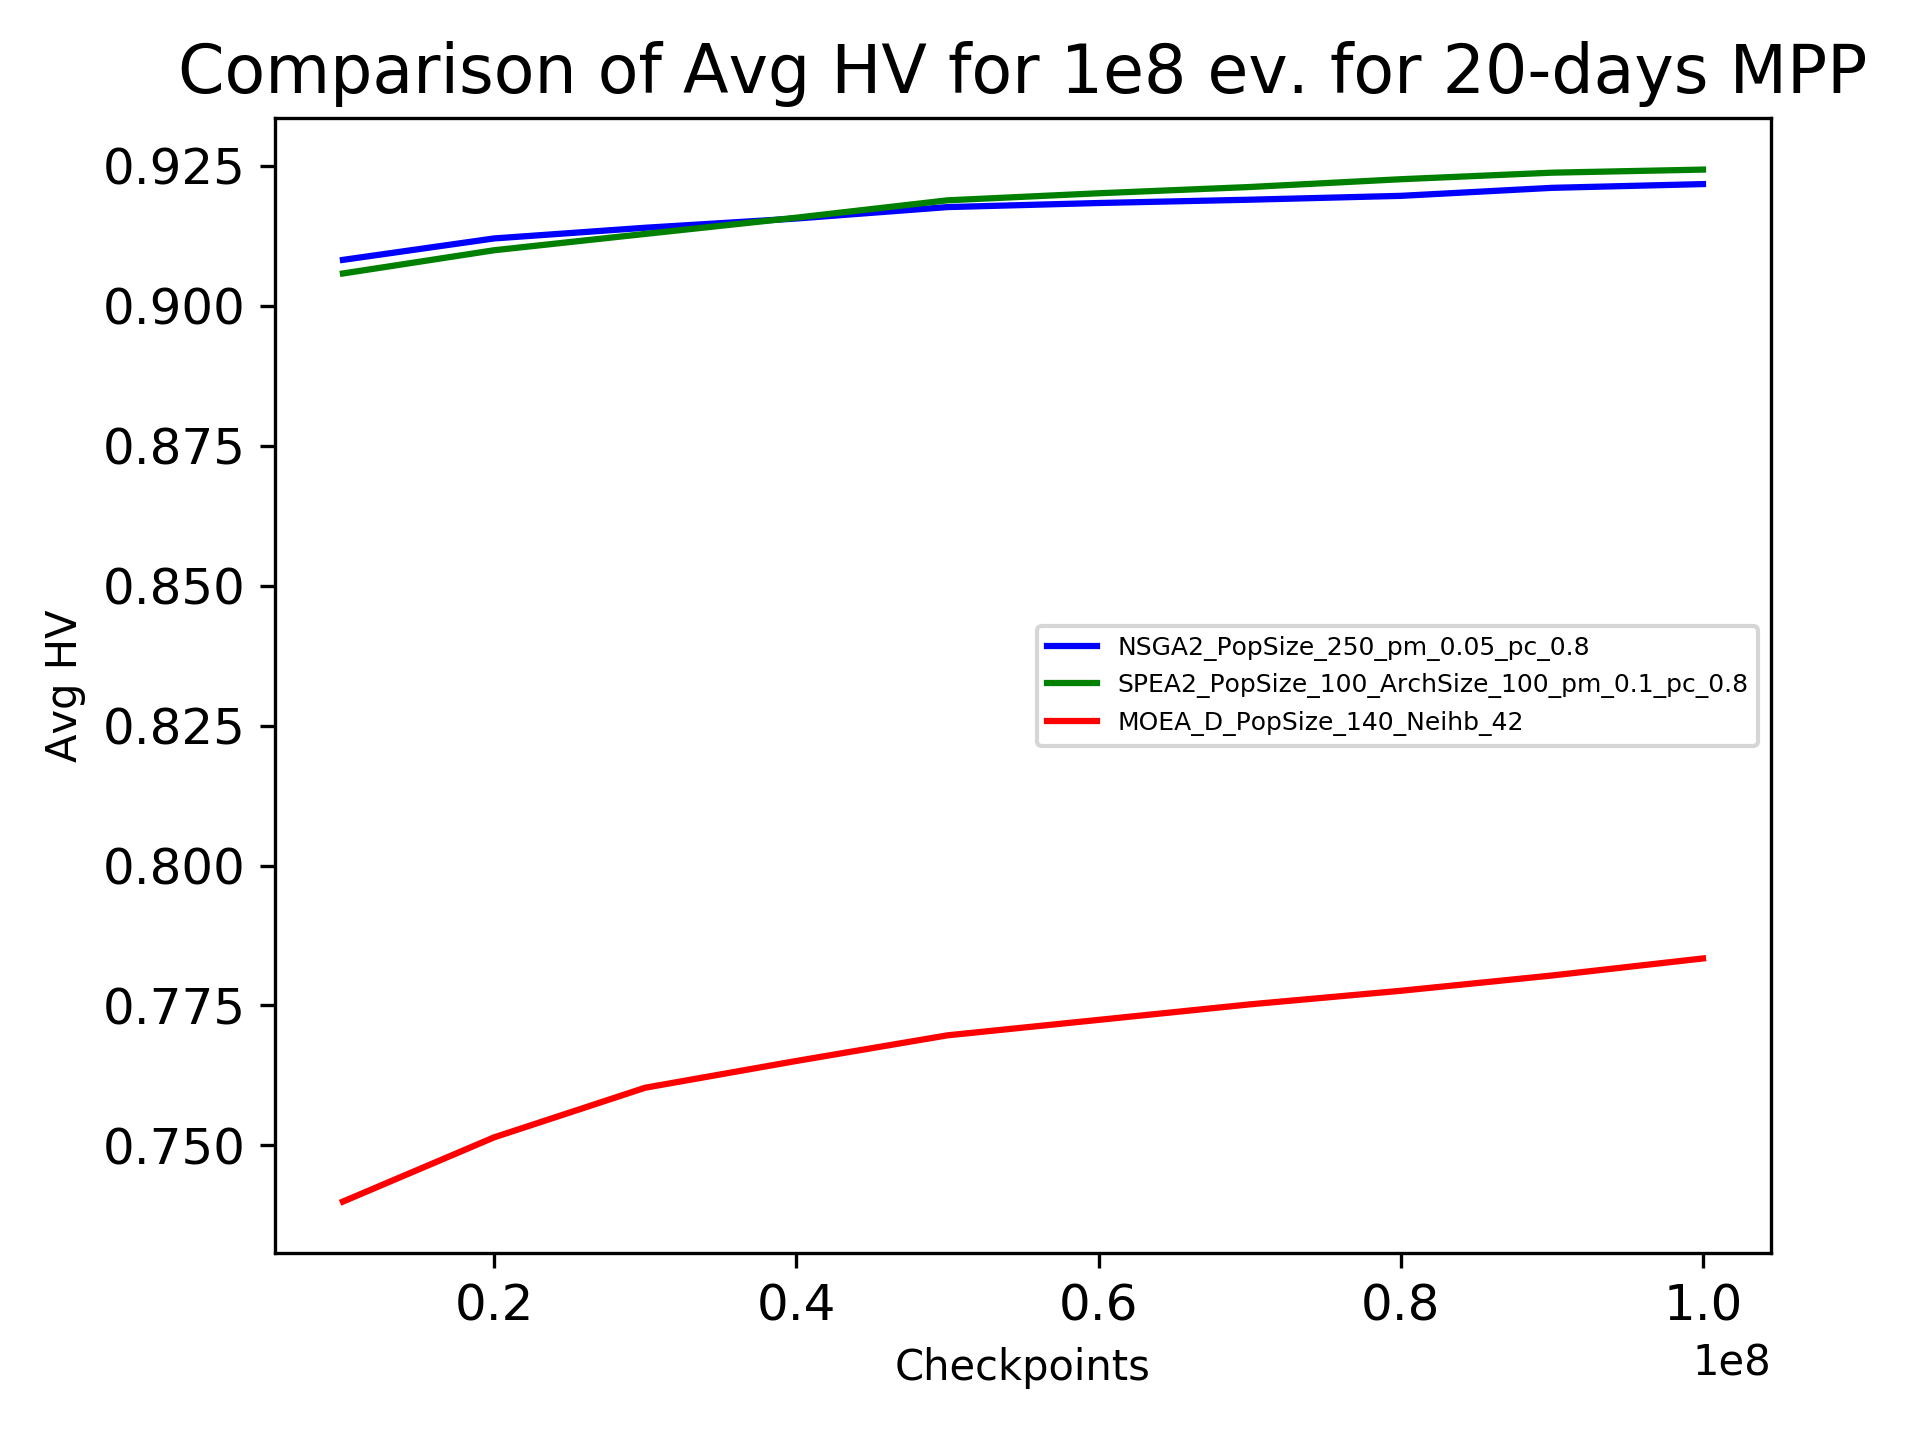
\includegraphics[width=1.0\linewidth]{images/avg_evolution_20_days.png}
\end{figure}
\end{frame}

\begin{frame}[fragile]{Variación del Tamaño del Problema.}
\begin{figure}
    \centering
    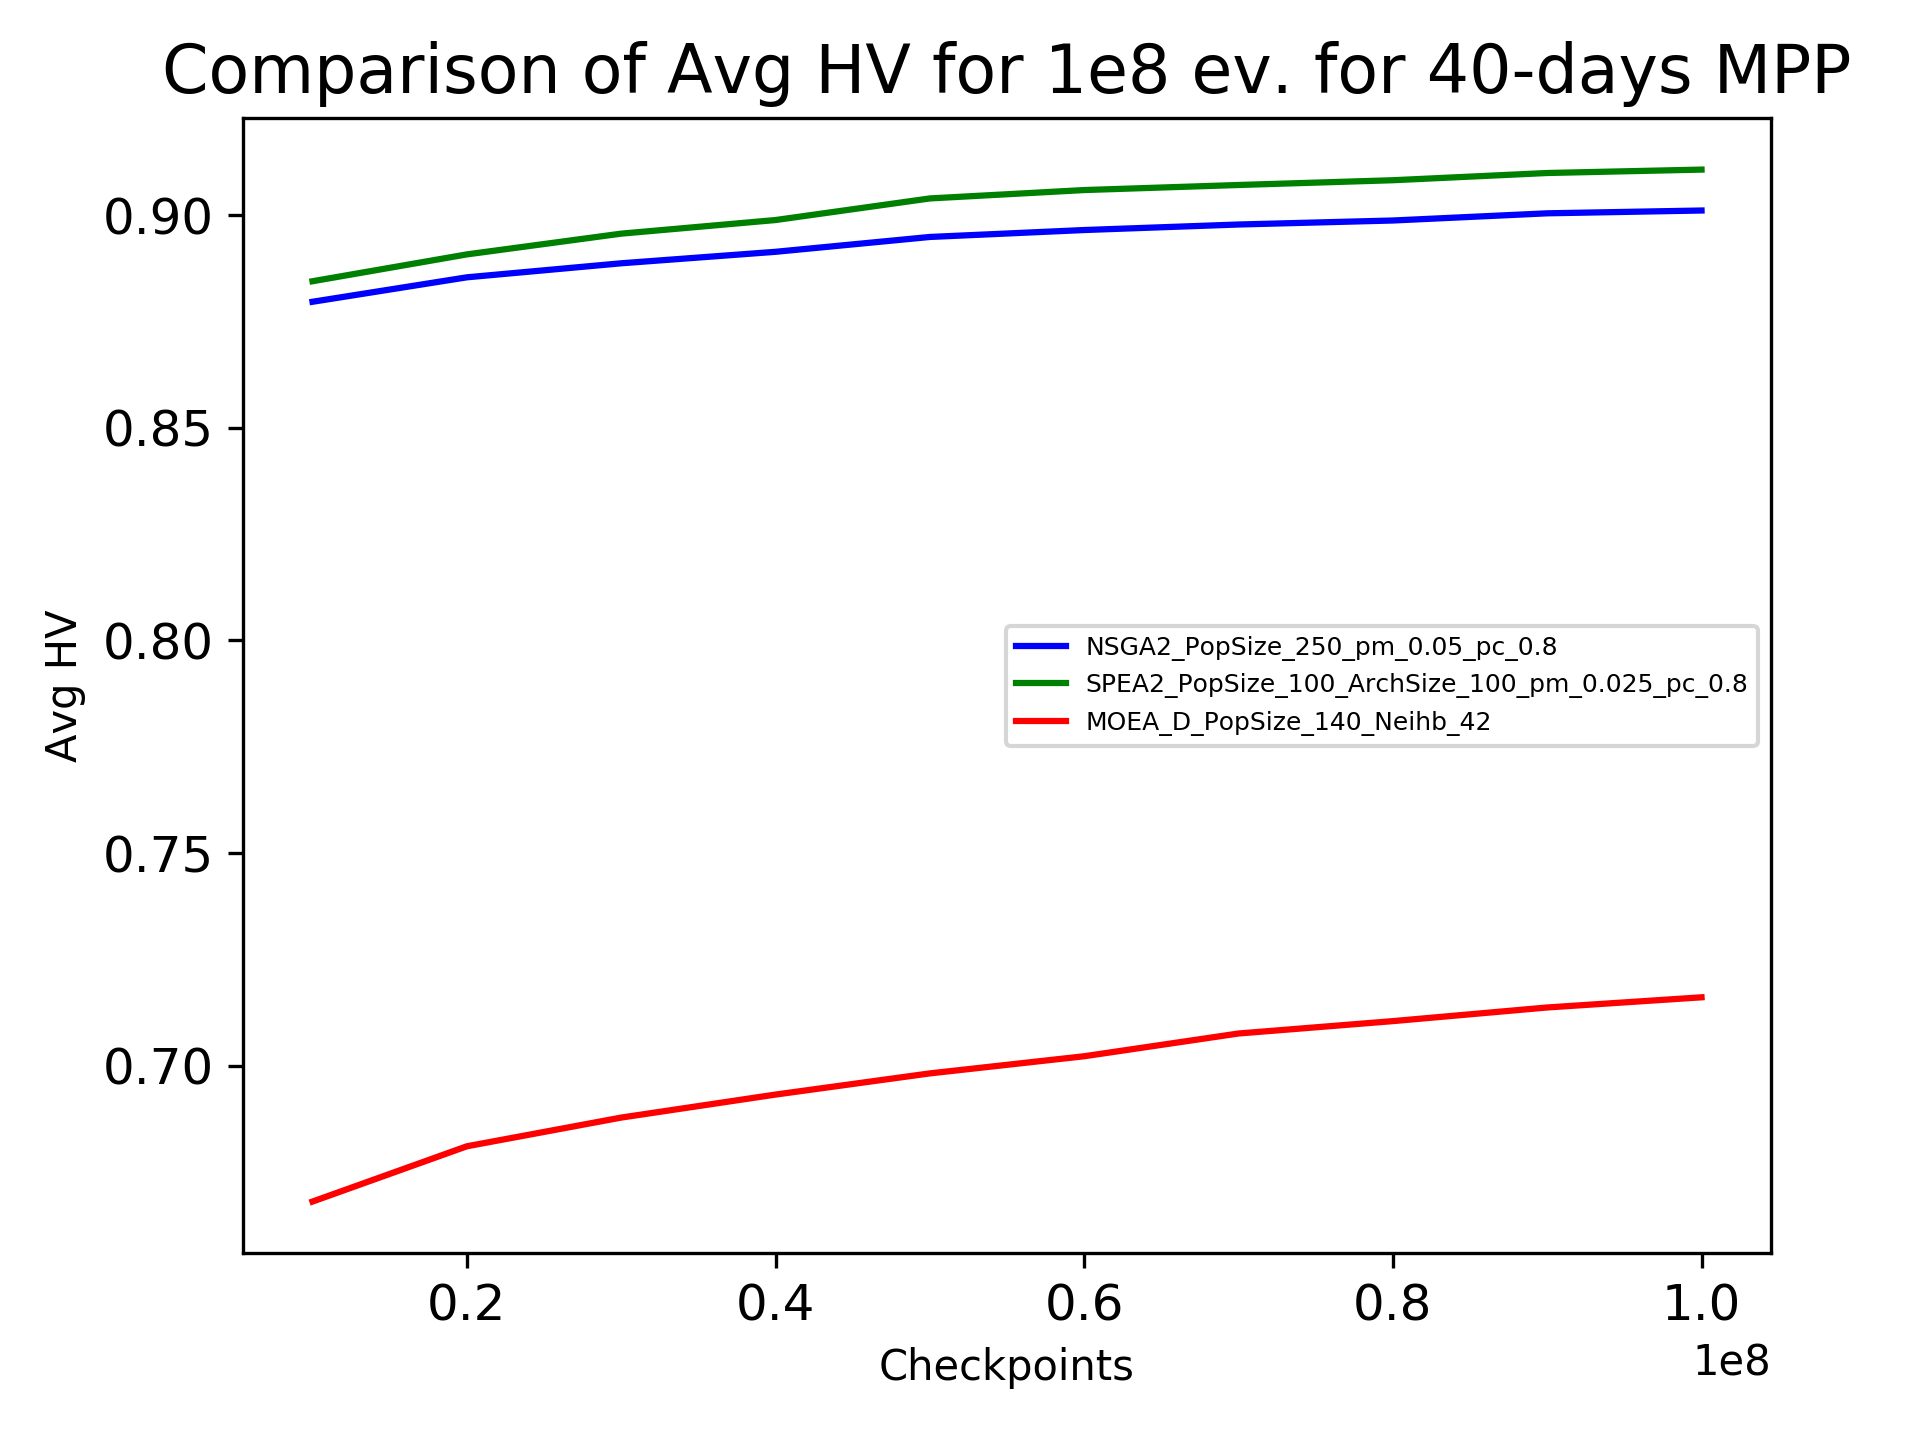
\includegraphics[width=1.0\linewidth]{images/avg_evolution_40_days.png}
\end{figure}
\end{frame}

%%%%%%%%%%%%%%%%%%%%%%%%%%%%%%%%%%%%%%%%%%%%%%%%%%%%%%%%%%%
% CONCLUSIONES
\section{Conclusions}
\begin{frame}[fragile]{Conclusions and Future Work.}
\begin{itemize}
    \item NSGA-II and SPEA-2.
    \item Quite simple MOEA/D.
\end{itemize}
Future work:
\begin{itemize}
    \item Initial weight generation.
    \item Other parameters.
    \item Increasing evaluation limit to 4e8.
    \item More configurations.
\end{itemize}
\end{frame}
%%%%%%%%%%%%%%%%%%%%%%%%%%%%%%%%%%%%%%%%%%%%%%%%%%%%%%%%%%%%

{\setbeamercolor{palette primary}{fg=white, bg=darkpastelpurple}
\begin{frame}[standout]
  ¿Preguntas?
\end{frame}
}

\begin{frame}[allowframebreaks]{References}

  \bibliography{slides}
\bibliographystyle{plain}

\end{frame}

\end{document}
